\chapter{Problématique du modèle d'intéressement \& Méthodologie}\label{chap:chapiter3}

\chaptermark{Problématique du modèle d'intéressement \& Méthodologie}
%\minitoc

L'écosystème OKP4, tout en apportant une structure pour l'économie de la connaissance, présente également des défis et des questions cruciales liés aux modèles économiques dans les zones. Le présent chapitre débute par une exposition des particularités du modèle économique au sein de l'écosystème OKP4 (\ref{subsec:modele_eco}), tout en soulevant la problématique inhérente au modèle d'intéressement financier (\ref{subsec:problem}). Par la suite, dans la \autoref{sec:methodologie}, la méthodologie adoptée pour fournir des éléments de réponse aux questions énoncées précédemment sera exposée.

\begin{comment}
    L'écosystème OKP4, tout en apportant une structure pour l'économie de la connaissance, présente également des défis et des questions cruciales liés aux modèles économiques dans les zones. Nous démarrons ce chapitre par une présentation des spécificités du modèle économique dans l'écosystème OKP4 (\ref{subsec:modele_eco}) et posons le problème d'un modèle d'intéressement financier (\ref{subsec:problem}). Par la suite,  dans la \autoref{sec:methodologie} nous exposerons notre méthodologie pour apporter des éléments de réponses aux questions posées précédemment.
\end{comment}

\section{Le modèle économique dans l'écosystème OKP4}\label{sec:modele_eco}

\subsection{Le modèle économique dans l'écosystème OKP4}\label{subsec:modele_eco}

\begin{comment}
Un modèle économique, dans l'écosystème OKP4, en tant que composante de la gouvernance d'une zone (\textit{Cf.} \ref{subsec:rulebook}), désigne la manière dont les agents économiques %gère, partage et%
captent de la valeur en partageant leurs ressources numériques (données, algorithmes, etc.) au sein de cette zone. Dans l'écosystème OKP4 le modèle économique d'une zone (*) s'articule autour d'une proposition de valeur centrée sur chaque connaissance créée. Dans cette économie de la connaissance, le modèle économique définit le mode de rémunérations des services qui ont servi à créer la connaissance, comment est calculé la valeur (monétaire) de la connaissance créée, comment est calculée la contribution de chaque agent économique qui participe en partageant ses données à la création d'une connaissance et la contrepartie (intellectuelle ou monétaire) qu'il reçoit à hauteur de cette contribution. Le modèle économique de chaque zone peut être customisé pour refléter et prendre en compte les objectifs et les intérêts de chaque participant de la zone. 
\end{comment}

Dans l'écosystème OKP4, le modèle économique au sein d'une zone joue un rôle central dans la gouvernance (\ref{subsec:rulebook}) en déterminant comment les acteurs économiques tirent de la valeur de leurs ressources numériques (comme les données et les algorithmes) partagées au sein de cette zone. Concrètement, il s'agit de la manière dont la valeur est capturée en échange du partage de ces ressources.

Ce modèle économique, spécifique à chaque zone, gravite autour d'une proposition de valeur centrée sur la création de connaissance. Dans ce contexte axé sur la connaissance, le modèle économique détermine comment rémunérer les services qui ont contribué à la création de la connaissance. Il définit également la façon de quantifier la valeur monétaire de cette connaissance nouvellement générée. De plus, il évalue la contribution de chaque acteur économique qui participe en partageant ses données pour la création de connaissance, et en retour, précise la récompense (qu'elle soit intellectuelle ou monétaire) en proportion de cette contribution.

Ces modèles économiques de zones peuvent être adaptés pour aligner les objectifs et les intérêts de chaque participant au sein de la zone, permettant ainsi une personnalisation en fonction des besoins spécifiques de chacun.
Un exemple concret est celui des agents $A$, $B$ et $C$ opérants dans deux zones distinctes, $Z_1$ et $Z_2$. Avec le protocole OKP4, les barrières techniques et réglementaires telles que la sécurité et la souveraineté des données sont éliminées. Cependant, l'alignement des intérêts économiques reste crucial. Dans la zone $Z_1$, $A$ et $B$ sont mutuellement intéressés par la connaissance générée grâce à la combinaison de leurs données. En revanche, dans $Z_2$, l'agent $B$ n'est incité à partager ses données avec $C$ que par des motivations financières. Si une autre entité, l'agent $D$, trouve de la valeur dans la connaissance issue de cette combinaison, $B$ et $C$ doivent être compensés financièrement. Ce cas d'étude démontre l'importance d'adopter des modèles économiques flexibles et adaptatifs dans les zones pour répondre aux besoins variés des participants en fonction des différents contextes de partage de données. Deux types de modèles sont ainsi mis en évidence et se distinguent par le type de contrepartie, ici intellectuelle ou financière, que reçoivent les contributeurs.

Selon que la contrepartie soit financière ou technique pour les agents qui partagent leurs données on distingue respectivement un modèle d'intéressement intellectuel et un modèle d'intéressement financier.

Dans un modèle économique, le modèle d'intéressement financier concerne les agents qui partagent leurs données dans la zone où ce modèle s'applique. Ce modèle définit explicitement la méthode utilisée pour calculer la valeur monétaire d'une connaissance, la méthode pour rédistribuer cette valeur monétaire entre les contributeurs de données une fois les services mis en oeuvre pour créer la connaissance et la méthode pour calculer la contribution marginale de chaque jeu de données ou agent.

\subsection{La problématique d'un modèle d'intéressement financier dans l'écosystème OKP4}\label{subsec:problem}

Dans l'écosystème OKP4, à l'ère de l'économie de la connaissance, les agents économiques peuvent collaborer pour créer une connaissance et recevoir une contrepartie financière à la hauteur de leur contribution selon la valorisation qui est faite de la connaissance  dans le cadre d'un modèle d'intéressement financier. Définir un modèle d'intéressement financier dans la gouvernance de la zone permet d'apporter de la transparence sur le mécanisme de valorisation d'une connaissance (prix), éviter la paralysie du vendeur, automatiser l'exécution des transactions évitant de longues négociations. Toutefois, la mise en place d'un tel modèle soulève des questions :  comment évaluer financièrement la connaissance dérivée d'un ensemble de jeux de données et services de traitement ? Comment rémunérer équitablement tous les agents qui ont partagé leurs données pour permettre la création de cette connaissance ? L'implémentation technique de ce modèle d'intéressement prenant la forme d'un programme informatique, il se pose également la question : est-ce que la complexité en temps de calcul et en espace de stockage du programme du modèle permet son implémentation sur les noeuds d'une blockchain ?

\subsubsection{Question 1 : La valeur de la connaissance}\label{subsubsec:q1}

L'évaluation financière  d'une connaissance est un défi en soi car, contrairement aux produits et services traditionnels, comme toute donnée, la connaissance n'a pas de coûts de production tangibles, et sa valeur peut être subjective, fluctuante et souvent difficile à quantifier. \citeauthor{agarwal_marketplace_2019} (\citeyear{agarwal_marketplace_2019}) résument quatre propriétés qui font des données des actifs uniques. 

Premièrement, les données peuvent être reproduites à un coût marginal nul. C'est par exemple le cas lors des actions "copier/coller".

Deuxièmement, la valeur des données est intrinsèquement combinatoire. Autrement,  les données ont une valeur qui est fondamentalement liée à leur capacité à être combinées ou analysées de différentes manières. 

Troisièmement, la valeur des données varie considérablement d'un acheteur à l'autre.

Enfin, l'utilité des données réside dans la valeur des informations qui en sont tirées, ce qui est difficile à vérifier a priori. En raison de ces propriétés, les modèles de tarification des biens physiques ne peuvent pas être directement appliqués ou étendus aux produits de données, et de nouveaux principes, théories et méthodes doivent donc être développés.

\subsubsection{Question 2 : Le calcul des contibutions}\label{subsubsec:q2}
Une fois la valeur de la connaissance établie, le défi suivant est de déterminer la contribution de chaque acteur à sa création. La contribution ne se limite pas seulement à la quantité de données fournies. Elle englobe également la qualité, la pertinence, les efforts de traitement de ces données, etc. . Dans l'écosystème OKP4, le calcul des contributions ne concerne que les fournisseurs de données. Les fournisseurs des services de traitements (infrastructures, programmes, etc.)  définissent le prix pour l'utilisation de leurs services.
Par exemple, si un service Google Cloud est référencé sur le protocole, l'utilisateur de ce service paye le coût d'exécution de ce service, fixé par son fournisseur. 

En effet, alors que la valeur d'un service de traitement est souvent définie par des coûts opérationnels, d'infrastructure et de maintenance, et est généralement fixée par le fournisseur du service, la donnée n'a pas de coût de production fixe et tangible. Si un service de traitement a un coût d'utilisation défini et prévisible, la connaissance requiert une approche d'évaluation plus fluide et adaptable, capable de prendre en compte les nuances, les spécificités de chaque contexte d'utilisation et permettre une rémunération juste des fournisseurs de données. Cette distinction est essentielle pour comprendre la dynamique de valorisation dans l'écosytème OKP4 et garantir une rémunération équitable pour tous les acteurs impliqués.

\subsubsection{Question 3 : La capacité pour une blockchain d'exécuter les algorithmes du modèle d'intéressement}\label{subsubsec:q3}

La problématique de la mise en place d'un modèle d'intéressement financier au sein des écosystèmes de partage de données se complexifie davantage lorsqu'il s'agit de l'implémenter sur blockchain. Bien que la blockchain offre une transparence, une traçabilité et une sécurité renforcées, elle pose également des défis techniques quant à sa capacité à exécuter des algorithmes complexes liés à un modèle d'intéressement.

La nature décentralisée des blockchains signifie que tout algorithme ou toute logique de contrat doit être exécuté sur chaque nœud du réseau, ce qui peut se traduire par des temps d'exécution plus longs, surtout si l'algorithme est complexe. De plus, les coûts associés à l'exécution de ces algorithmes, souvent payés en crypto-monnaie native de la blockchain, peuvent s'avérer prohibitifs, surtout si l'algorithme nécessite beaucoup de puissance de calcul.

Implémenter le modèle d'intéressement dans la blockchain, malgré les défis techniques potentiels, peut donc offrir une assurance supplémentaire de l'intégrité, de la transparence et de l'équité du processus pour tous les participants. Cela pourrait, en fin de compte, favoriser une adoption plus large du modèle parmi les acteurs, en renforçant la confiance et en réduisant les risques perçus associés au partage de données.\\

\\
\begin{comment}
   Dans les prochaines parties, nous allons présenter une méthodologie pour répondre à ces trois questions avant d'en exposer les résultats. 
\end{comment}


\section{Méthodologie}\label{sec:methodologie}


\subsection{Modélisation du problème} \label{subsec:model_pb}

La modélisation se présente comme une étape cruciale dans la compréhension approfondie de la problématique relativement complexe adressée dans cette étude, concernant l'évaluation financière de la connaissance et le calcul de la valeur de chaque contribution de sa création dans les écosystèmes de partage de données. Il est important d'établir des relations claires entre les composantes clés du modèle d'intéressement financier afin de créer un cadre structuré qui facilite l'isolement, l'analyse et la résolution de sous-problèmes spécifiques.

\subsubsection{La connaissance} \label{subsubsec:connaissance}

La connaissance, dans l'écosystème OKP4 désigne l'information qui est produite à la suite de la mise en commun de plusieurs données et leurs aggrégation. Dans la pratique une connaissance peut être le fruit de la jointure puis de l'aggrégation de plusieurs données. C'est le cas lorsqu'on calcule la moyenne sur un ensemble de données ou encore pour le calcule d'un indicateur plus élaboré comme l'indice de fréquence de traitement (IFT), en agriculture, à partir de plusieurs jeux de données. Et la moyenne, et l'IFT sont des connaissances.  Dans la suite, la valeur de la connaissance est calculé sur le résultat de la jointure car à l'étape d'aggrégation il est difficile, voire impossible, de remonter aux contributions de chacun quant à la qualité de l'information apporté. La considération du résultat de la jointure avant l'agrégation, désignée ultérieurement par <<connaissance>> par abus de langage dans le cadre de cette analyse, s'inscrit dans le principe du "\textit{shit in, shit out}" \footnote{"Entrées médiocres, sorties médiocres"}.

\begin{comment}
    Le fait de considérer le résultat de la jointure avant l'aggrégation, que dans la suite nous appelerons connaissance par abus de langage, pour notre analyse se tient selon le principe du "\textit{shit in, shit out}" \footnote{"Entrées médiocres, sorties médiocres".}.
\end{comment}


\begin{comment}
\begin{figure}
    \centering
    %\includegraphics{}
    \caption{shéma de jointure}
    \label{fig:}
\end{figure}
\end{comment}


\subsubsection{Knowledge Marketplace} \label{subsubsec:kg_marketplace}

On se positionne dans une zone $Z$ au sein du \textit{dataverse}, avec un intérêt porté à une situation où un ensemble de $N_0$ jeux de données $D_0 = \{D_{0,1}, D_{0,2}, D_{0,3}, ... D_{0,N_0}\}$ provient de $P_0$ fournisseurs de données distincts $F_0 =\{F_{0,1}, F_{0,2}, F_{0,3}, ... F_{0,P_0}\}$, et est employé pour la création de la connaissance $K_{G_0}$ via une série de services de traitement notés simplement $S_0$. Étant donné que $N_0$ peut différer de $P_0$, cette étude se concentre uniquement sur les jeux de données pour les analyses ultérieures. En effet, un fournisseur de données $F_{0,k}$ de $F_0$ peut contribuer avec plusieurs données dans $D_0$. La figure \ref{fig:first_side_market_place} permet d'illustrer cette phase de création de la connaissance. À ce stade, chaque donnée présente dans $D_0 $ ne possède pas encore de valeur marchande, car la connaissance produite n'a pas encore été valorisée.

\begin{comment}
    Nous nous plaçons dans une zone $Z$ du dataverse et nous nous intéressons à une situation où un ensemble de $N_0$ jeux de données $D_0 = \{D_{0,1}, D_{0,2}, D_{0,3}, ... D_{0,N_0}\}$, de $P_0$ fournisseurs de données distincts $F_0 =\{F_{0,1}, F_{0,2}, F_{0,3}, ... F_{0,P_0}\} $, est utilisé pour créer la connaissance $K_{G_0}$ via une série de services de traitement que nous notons simplement $S_0$. $N_0$ n'étant pas nécéssairement égale à $P_0$, nous ne considérons que les jeux de données dans le reste de nos analyses. En effet, un fournisseur de données $F_{0,k}$ de $F_0$ peut fournir plusieurs données dans $D_0 $. La figure \ref{fig:first_side_market_place} permet de visualiser cette phase de création de la connaissance. A ce stade chaque donnée de $D_0 $ n'a aucune valeur marchande puisque la connaissance produite n'a pas encore été valorisée.
\end{comment}

\begin{figure}[h]
    \centering
    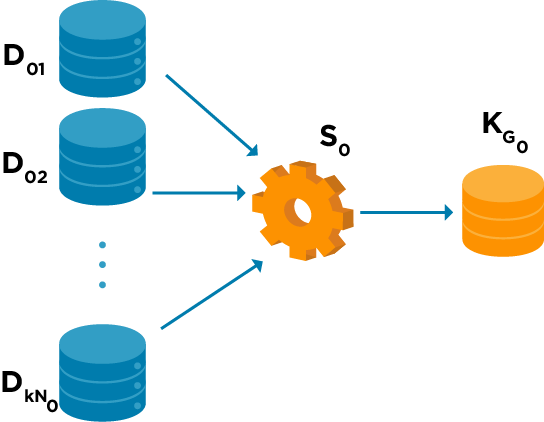
\includegraphics[width=0.3\textwidth]{ILLUSTRATIONS/graph_k0.png}
    \caption{Phase de création de la connaissance}
    \label{fig:first_side_market_place}
\end{figure}


En fait, la connaissance $K_{G_0}$ sera produite à l'initiative d'un consommateur de connaissance $C_{0,1}$. $C_{0,1}$ n'a pas un accès exclusif à la connaissance. Notons $C_0 = \{C_{0,1}, C_{0,2}, ... C_{0,T_0}\}$ les $T_0$ consommateurs successifs de $K_{G_0}$.

Outre ce qui doit servir pour rémunérer la série de services de traitement $S_0$, $C_{0,t}$, le $t^{eme}$ consommateur de la connaissance, payera le prix calculé $V_{K_{G_{0,t}}}$, la valeur de la connaissance calculé pour ce consommateur. Cette seconde phase fonctionne comme une data marketplace classique, dans la zone $Z$ à la différence que $V_{K_{G_{0,t}}}$ est calculé dynamiquement (\ref{subsubsec:kg_value}). la figure \ref{fig:scnd_side_market_place} permet de visualiser cette phase de valorisation de la connaissance.


\begin{figure} [h]
    \centering
    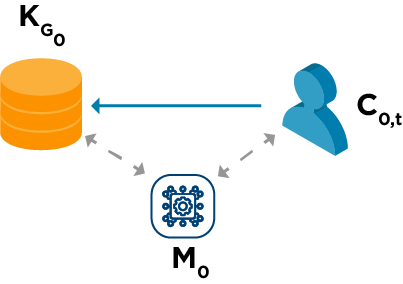
\includegraphics[width=0.25\textwidth]{ILLUSTRATIONS/market_k0_update.png}
    \caption{Valorisation de la connaissance auprès d'un consommateur}
    \label{fig:scnd_side_market_place}
\end{figure}

Les deux phases mises bout à bout permettent d'obtenir une <<chaîne de valeur>> de la connaissance $K_{G_0}$ comme schématisé sur la \ref{fig:market_place}.

\begin{figure}[h]
    \centering
    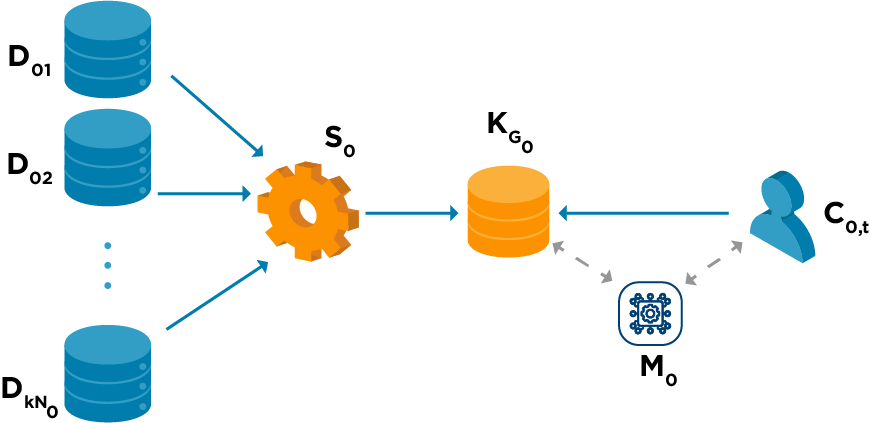
\includegraphics[width=0.5\textwidth]{ILLUSTRATIONS/kg_graph_k0.png}
    \caption{Chaîne de valeur de la connaissance $K_{G_0}$}
    \label{fig:market_place}
\end{figure}

Sur cette figure, $M_0$ désigne une marketplace, celle de la connaissance produite : c'est une \textit{knowledge marketplace}\footnote{place de marché de la connaissance.}. Dans la suite, le terme \textit{marketplace} est utilisé pour faire référence au système de programmes informatiques qui automatisent le modèle d'intéressement.  C'est au niveau de la \textit{marketplace} que se font les calculs pour le modèle d'intéressement: le calcul de la valeur de la connaissance, le calcul des contributions et la redistribution de la valeur générée au prorata des contributions calculées.



\begin{comment}

La marketplace $M_0$ calcule $V_{K_{G_{0,t}}}$, reçoit le paiment de $C_{0,t}$ et partage $V_{K_{G_{0,t}}}$ entre les données de $D_0$ au prorata de leurs contributions : la phase de rétribution.


\textbf{Remarque} : Les jeux de données pouvant prendre des formes et des formats variés, nous considérons ici que chaque jeu de données est sous forme tabulaire et que la connaissance obtenue par jointure l'est aussi.
     et les transactions entre les fournisseurs de données, fournisseurs de services et consommateurs de connaissances
     
Remarque : La valeur que $C_0$ serait prêt à payer pour la connaissance dépend de son évaluation personnelle.

    Remarque : Cette marketplace peut s'apparenter à un système d'enchère en une étape dans lequel l'acheteur arrive fait une offre, et repart immédiatement avec une version de la connaissance (Ssec Explication du dispositif).
    Remarque : Dans l'Ecosystème OKP4, les fournisseurs de données ne maximisent pas nécessairement leurs revenus dès leurs premières utilisation.

\end{comment}

\begin{comment}
    \begin{figure}
    \centering
    %\includegraphics{}
    %\caption{Caption} un schéma qui montre un flux d'argent
    \label{fig:market_place_partage}
\end{figure}
\end{comment}


\subsubsection{Graphe de connaissances} \label{subsubsec:kg_graph}

Dans le dataverse, une connaissance $K_G$ produite peut être réutilisée comme donnée d'entrée dans la création d'une autre connaissance. Par exemple ${K_{G_0}}$ peut intervenir dans la création d'une connaissance ${K_{G_1}}$ avec un ensemble de $N_1$ jeux de données $D_1 = \{D_{1,1}, D_{1,2}, D_{1,3}, ... D_{1,N_1}\}$ via une série de traitements $S_1$. Par le même mécanisme on peut aboutir à la création d'une connaissance ${K_{G_k}}$ mettant en jeu $D_k = \{D_{k,1}, D_{k,2}, D_{k,3}, ... D_{k,N_k}\}$, une connaissance ${K_{G_{k-1}}}$ et $S_k$ comme le montre la figure \ref{fig:kg_graph}.

Le graphe de la figure \ref{fig:kg_graph} constitue le graphe de connaissances (knowledge graph) et retrace la généalogie de la connaissance ${K_{G_k}}$ dans la zone $Z$ du dataverse. ${K_{G_{k-1}}}$, $D_k$ et $S_k$ sont les ressources utilisées pour la création de la connaissance au \textbf{rang} $k \geq 1$. Au rang 0, $D_0$ et $S_0$ sont mis en jeu.

\begin{comment}
    , d'un ensemble de $P_1$ fournisseurs de données distincts $F_1 =\{F_{1,1}, F_{1,2}, F_{1,3}, ... F_{0,P_1}\}$,
    fournis par $F_k =\{F_{k,1}, F_{k,2}, F_{k,3}, ... F_{k,P_k}\}$,
\end{comment}

\begin{figure}[H]
    \centering
    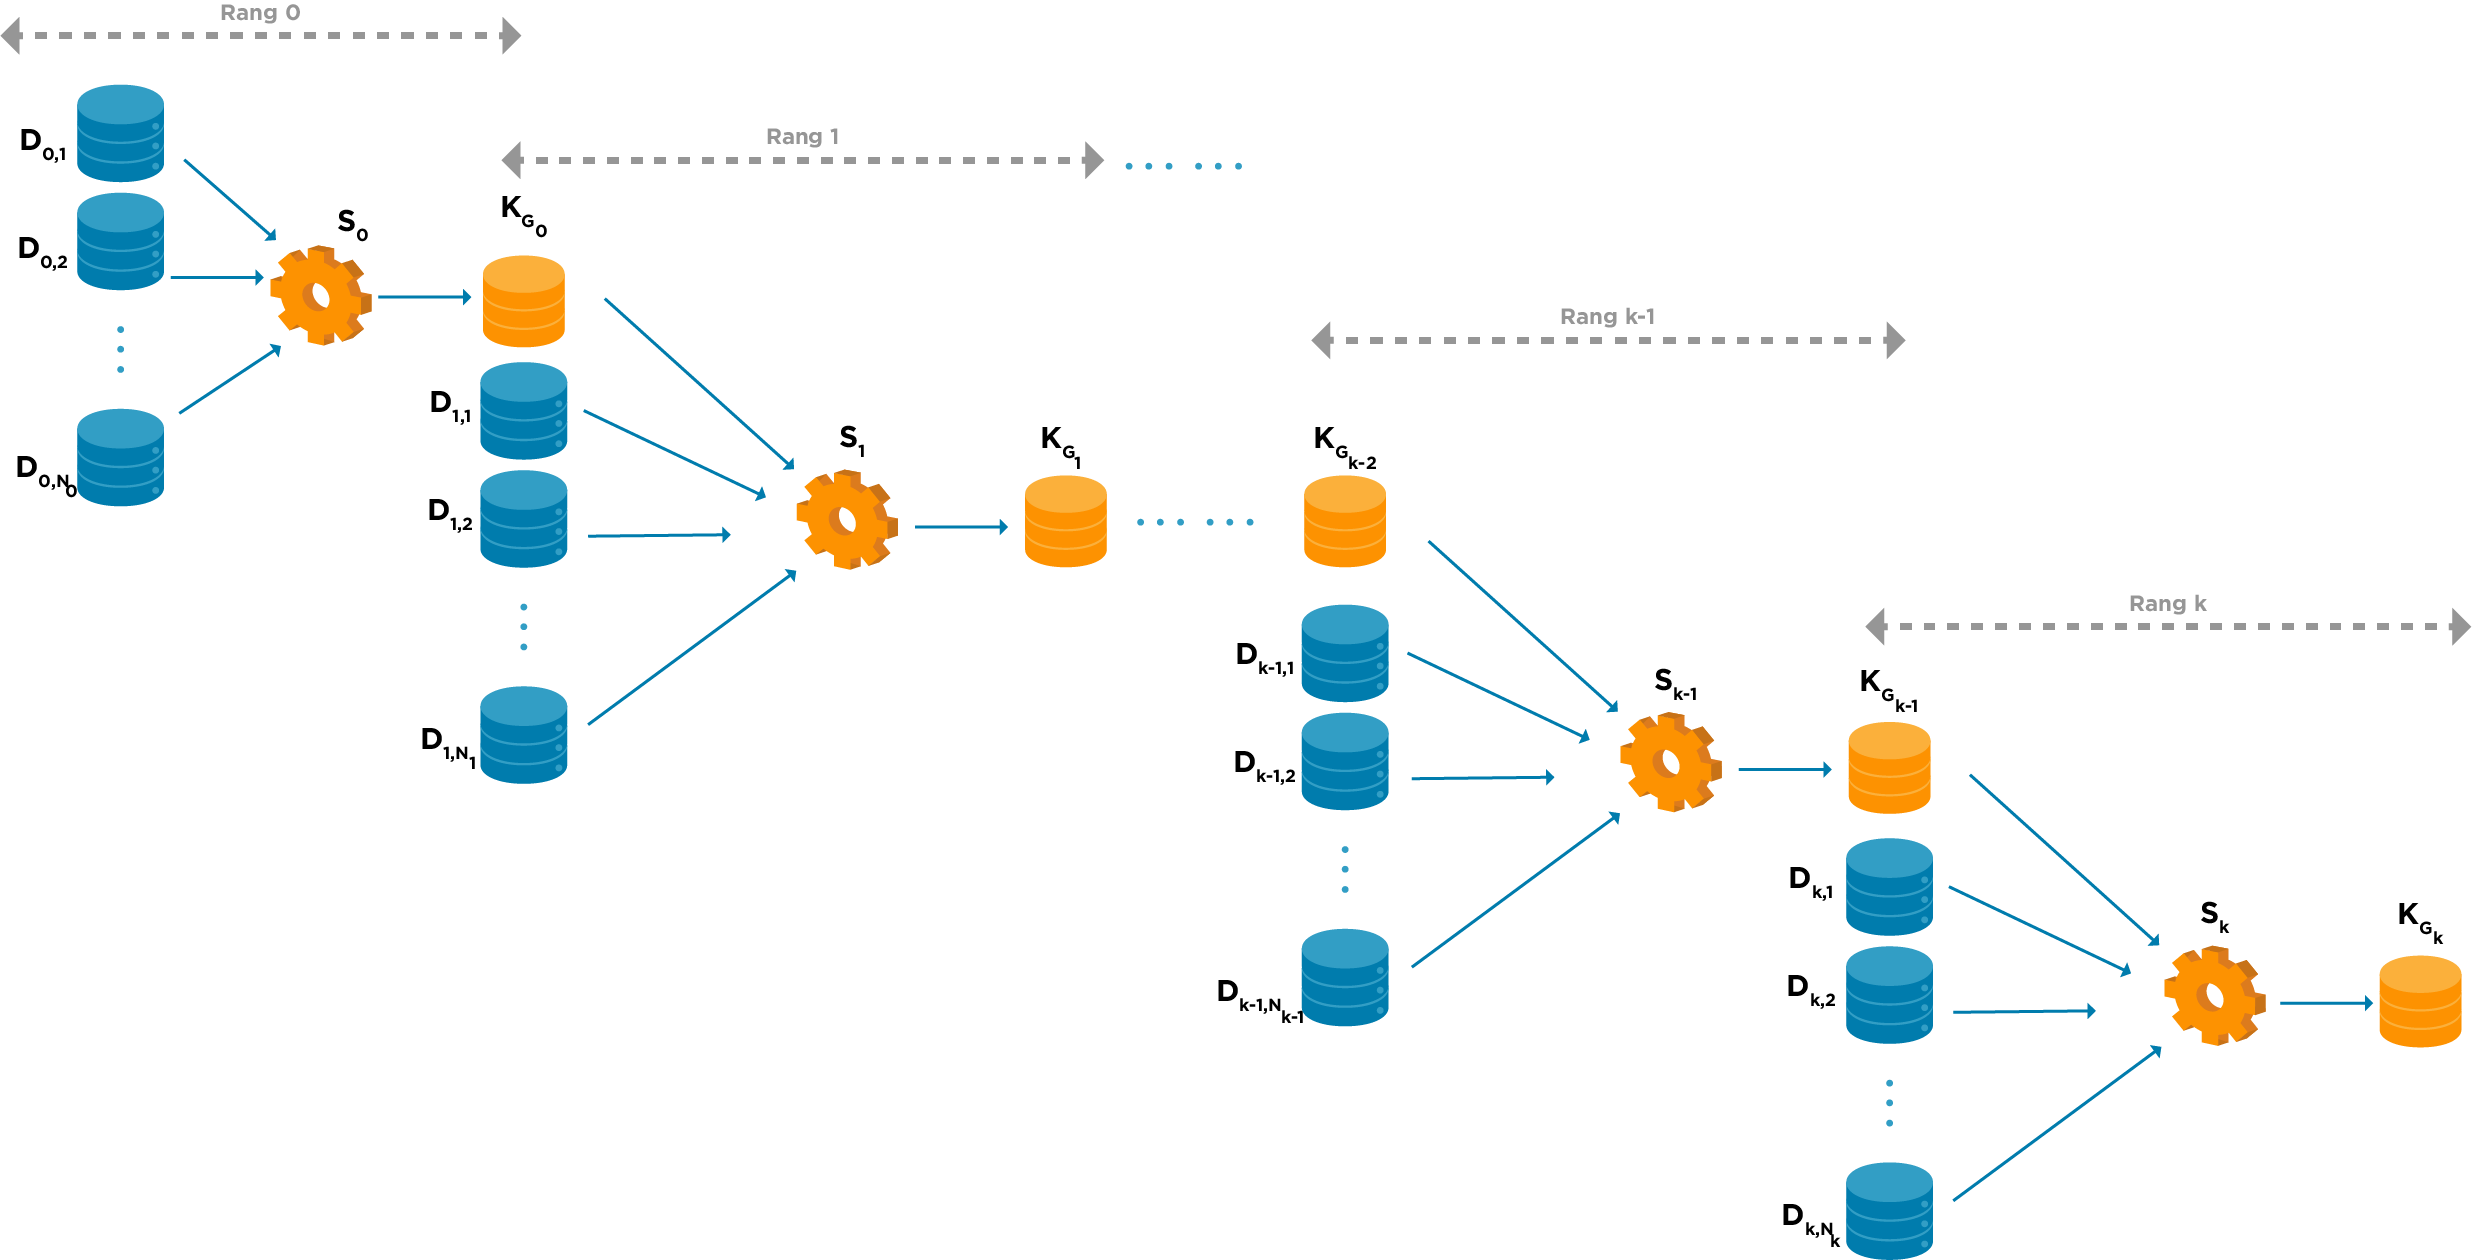
\includegraphics[width=0.8\textwidth]{ILLUSTRATIONS/kg_graph.png}
    \caption{Graphe de connaissances}
    \label{fig:kg_graph}
\end{figure}


%\subsection{Interactions dans le dataverse} \label{subsec:marketplace}
%Dans le dataverse cinq types d'agents économiques interagissent:  les fournisseurs de services, les fournisseurs de données, les validateurs, les consommateurs et la marketplace dans un scénario décrit sur la figure \ref{fig:interactions}

%\begin{figure}
    %\centering
    %\includegraphics{}
    %\caption{Caption}
    %\label{fig:interactions}
%\end{figure}


%\section{Cadrage théorique}\label{sec:current_state}

%Pour ne pas reinventer la roue, il est important 

%\section{Outils et implémentation}\label{sec:current_state}
\subsection{Travaux connexes}\label{subsec:travaux_connexes}

Cette étude, qui s'intéresse à la valorisation des connaissances dans l'écosystème OKP4, s'inscrit dans le champ plus large de la tarification des données, un domaine en pleine expansion. La complexité de la question traitée en matière de tarification des données positionne ce domaine à l'intersection de plusieurs disciplines, notamment la théorie de l'information, la théorie des enchères et la théorie des jeux, comme c'est le cas dans cette étude.

La théorie de l'information a été développée initialement par Claude Shannon en 1948. Elle est principalement concernée par la quantification de l'information. Cette théorie est utilisée pour comprendre comment l'information peut être encodée et transmise de manière efficace. Dans le contexte de la tarification des données, comprendre la "valeur de l'information" peut être crucial. Par exemple, certaines données peuvent être plus "informatives" que d'autres, et donc plus précieuses. Parmi les auteurs qui empruntent des outils de la théorie de l'information pour résoudre des problèmes de tarification de données il est possible de citer \citeauthor{deep_qirana_2017} (\citeyear{deep_qirana_2017}). Dans son analyse intitulé <<\textit{QIRANA: a Framework for Scalable Query Pricing}>> \citeauthor{deep_qirana_2017} s'intéressent à la tarification de requêtes d'une base de données. L'entropie de Shannon sert ici à quantifier le taux de rédondance dans les nouvelles requêtes par rapport aux anciennes : les requêtes redondantes ne sont pas facturé et le prix de la requête est donnée par la valeur de l'entropie de Shannon.

La théorie des enchères étudie comment les biens et les services sont alloués par le mécanisme des enchères. Cette théorie cherche à comprendre les stratégies optimales pour les acheteurs et les vendeurs sous différentes règles d'enchère. Les théoriciens des enchères, tels que William Vickrey, ont développé des modèles pour différents types d'enchères comme les enchères anglaises, hollandaises, et de Vickrey. Dans le domaine de la tarification des données, la théorie des enchères peut être utilisée pour déterminer comment les données peuvent être vendues au prix le plus élevé possible tout en étant équitable pour tous les participants. L'on rencontre l'usage d'outils dévéloppés dans le cadre de cette théorie dans les travaux de \citeauthor{agarwal_marketplace_2019} (\citeyear{agarwal_marketplace_2019}) et \citeauthor{mehta_how_nodate} (\citeyear{mehta_how_nodate}). Ces auteurs dans leurs deux études utilisent le modèle d'enchère optimale de \citeauthor{myerson_optimal_1981} (\citeyear{myerson_optimal_1981}) pour respectivement calculer les revenues à allouer aux fournisseurs de données pour l'entraînement d'un modèle de \textit{machine learning} et le prix d'une base de données.

La théorie des jeux est une branche des mathématiques qui étudie les interactions stratégiques entre différents <<joueurs>> ou agents dans un environnement donné. La théorie des jeux peut être coopérative ou non coopérative, et elle a été utilisée dans une multitude de domaines allant de l'économie à la biologie. Dans le contexte de la tarification des données, la théorie des jeux peut aider à comprendre comment différents agents (comme les acheteurs et les vendeurs de données) interagissent stratégiquement. Des concepts comme la <<valeur de Shapley>> peuvent être utilisés pour diviser équitablement la valeur générée par une coalition de fournisseurs de données. les travaux de \citeauthor{agarwal_marketplace_2019} (\citeyear{agarwal_marketplace_2019}) et \citeauthor{khan_incentive_2023} (\citeyear{khan_incentive_2023}) sont des cas d'application du concept de la valeur de \citeauthor{l_s_shapley_value_1952} à l'allocation équitable de ressources entre plusieurs fournisseurs de données.

Les travaux présentés ci-dessus ne sont qu'un aperçu de la diversité des approches qu'il existe en tarification des données et allocation de ressources entre fournisseurs de données. Dans <<\textit{Data Pricing in Machine Learning Pipelines}>> \citeauthor{cong_data_2021} présente une photographie plus étendue des pratiques qui existent dans le domaine de la tarification des données. Ces pratiques diverses et variées dépendent du type de données traitées et des hypothèses de départ.

L'approche exposée dans les prochaines sections s'appuie sur les modèles de plusieurs des travaux suscitées notamment ceux de \citeauthor{mehta_how_nodate} (\citeyear{mehta_how_nodate}) et \citeauthor{agarwal_marketplace_2019} (\citeyear{agarwal_marketplace_2019}). Toutefois, la présente étude est motivée par plusieurs considérations :

\begin{enumerate}
    \item Certaines études rencontrées dans la littérature sur le sujet supposent que le fournisseur de donnée est capable de fixer un prix de base sur sa base de données comme c'est le cas avec l'analyse de \citeauthor{deep_qirana_2017}. A contrario la présente étude s'intéresse à un scénario dans lequel le fournisseur n'a aucune idée de ce que vaut ses données ;
    \item \citeauthor{mehta_how_nodate} analyse un cas d'échange de données contre rémunération en supposant que le consommateur peut filtrer les données et sélectionner celles qui sont d'intérêt pour lui. A contratrio le cadre de cette étude se situe dans l'économie de la connaissance et pour des questions de confidentialité et souveraineté, il n'est pas possible de filter les données. Seule la connaissance est accessible selon le modèle du <<\textit{take all leave all}>>. 
\end{enumerate}

\subsection{Conception du modèle d'intéressement}\label{subsec:conc_mod_int}


\subsubsection{Valeur de la connaissance} \label{subsubsec:kg_value}

Considérons un rang $k$ du knowledge graph. L'objectif est de calculer la valeur monétaire $V_{K_{G_{k,t}}}$ de la connaissance $K_{G_k}$, au niveau d'une instance de marketplace $M_k$, que doit payer le consommateur $C_{k,t}$ pour y accéder. La création de $K_{G_k}$ met en jeu les ressources de $D_k$, de $S_k$ et la connaissance $K_{G_{k-1}}$ comme illustré sur la figure \ref{fig:market_place_vkg}\footnote{$K_{G_{k-1}}$ correspond à $D_{k,1}$ dans la figure \ref{fig:market_place_vkg}}.

\begin{figure}[h]
    \centering
    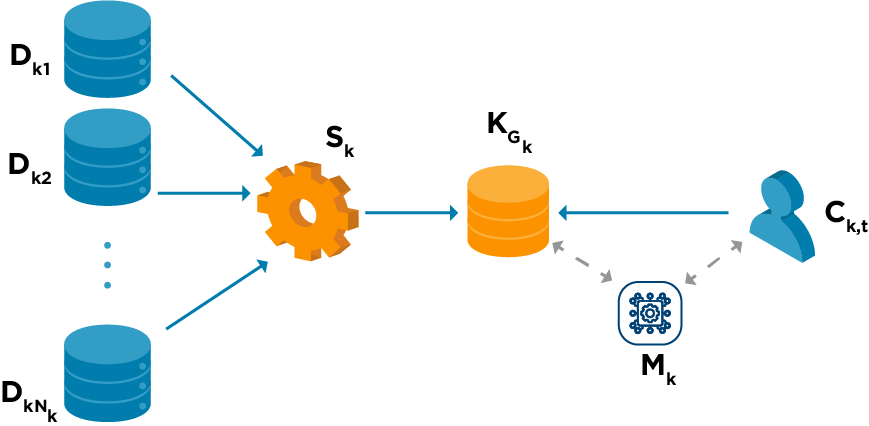
\includegraphics[width=0.5\textwidth]{ILLUSTRATIONS/kg_graph_kk_update_1.png}
    \caption{Rang k du graphe de connaissance}
    \label{fig:market_place_vkg}
\end{figure}

Enonçons ici quelques points importants, qui font office de contraintes dans l'évaluation de la valeur d'une connaissance :
\begin{enumerate} 
    \item \textbf{Contrainte 1:} La marketplace veut vendre le droit de consommer la connaissance au meilleur prix pour les fournisseurs de données mais ne sait pas combien les consommateurs potentiels seront prêt à payer ; \label{contrainte:1}
    \item \textbf{Contrainte 2:} Seul le consommateur de la connaissance à une meilleur idée des bénéfices que peuvent lui apporter la connaissance et des coûts qu'il peut se permettre pour l'avoir ; \label{contrainte:2}
    \item \textbf{Contrainte 3:} Dans la collection des consommateurs successifs, chacun à une évalution personnelle de la valeur monétaire de la connaissance ; \label{contrainte:3}
    \item \textbf{Contrainte 4:} Le prix total qu'est prêt à payer un consommateur de connaissance pour la quantité disponible dépend de sa  qualité. \label{contrainte:4}
\end{enumerate}
\begin{comment}
    $V_{K_{G_{k,t}}}$ doit tenir compte de la valeur subjective qu'a $C_{k,t}$ de la connaissance, de la qualité de l'information qu'elle apporte \footnote{Nous ne tenons pas compte de la quantité lors de l'évaluation de la valeur de la connaissance, car celle-ci est constante.}. $V_{K_{G_{k,t}}}$ doit en outre permettre de maximiser le revenu des fournisseurs de données de $F_k$ pour cette transaction (Ssec modélisation). De même $C_{k,t}$ à pour objectif de minimiser son coût d'acquisition de la connaissance.
\end{comment}

Pour simplifier la notation, les termes $V_{K_{G_{k,t}}}$ et $C_{k,t}$ sont respectivement abrégés en $V_t$ et $C_t$.

Des éléments permettant de déterminer $V_t$ en respectant les contraintes \ref{contrainte:1} et \ref{contrainte:2} ont été identifiés dans la littérature, notamment avec \cite{myerson_optimal_1981}. Dans son analyse, \citeauthor{myerson_optimal_1981} considère le problème d'une personne qui a un objet à vendre et qui ne sait pas combien ses acheteurs potentiels sont prêts à payer pour cet objet. Il propose une enchère optimale en réponse à ce problème. Par la suite, une tentative est faite pour appliquer les conclusions de cette recherche au problème adressé dans cette étude. Le système d'enchères qui sera développé possède une particularité : les consommateurs de la connaissance interviennent successivement, créant ainsi une enchère indirecte entre eux. Les résultats présentés dans \cite{myerson_optimal_1981} permettent de répondre aux 2 autres contraintes (\ref{contrainte:3} - \ref{contrainte:4}) énoncées précédemment.

Si l'on définit $Q(K_{G_k})$ comme étant la mesure de la qualité de la connaissance, alors la valeur que $C_t$ pense pouvoir en tirer est :

\begin{equation} \label{eq:vkg_q}
    V_t= \mu_t \cdot Q(K_{G_k})
\end{equation}

Cette équation \ref{eq:vkg_q} montre que $V_t$ est d'autant plus élevé que la qualité de la connaissance ($Q(K_{G_k})$) est élevée. Dans l'équation \ref{eq:vkg_q} $\mu_t$ est une information privée de $C_t$ ;  ce n'est donc pas $\mu_t$ qu'il va déclarer à la marketplace mais bien une valeur $b_t < \mu_t$ de sorte à minimiser ses coûts et maximiser son utilité \footnote{L'utilité est un concept fondamental en économie qui représente la satisfaction ou le plaisir que quelqu'un ressent en consommant des biens et des services.}. Notons que l'équation \ref{eq:vkg_q} permet de respecter la contrainte \ref{contrainte:4}.

Avant l'arrivée de $C_t$, la marketplace aura fixé un prix $p_t$ pour chaque unité de $Q(K_{G_k})$. $p_t$  doit être vu comme le prix de réserve du système d'enchère. Seulement, dans le modèle de cette étude, la connaissance est quand-même transmise à $C_t$, même si $b_t < p_k$, dans les conditions abordées en \ref{par:alteration_func}. 

\begin{comment}
   Tenir compte de la contrainte \ref{contrainte:2} pose un enjeu qui est alors d'inciter $ C_t$ à déclarer $b_t$ assez proche de $\mu_t$ afin de maximiser la rémunération des fournisseurs de données.  
\end{comment}

Le système en cours de construction nécessite que $p_k$ soit mis à jour de sorte à converger vers $p*$, la vraie valeur de la connaissance sur la population de ses consommateurs (\ref{par:prix_de_reserve_update}).

\paragraph{Valeur de la connaissance : une fonction de paiement de Myerson\\} \label{par:valeur_kg_myerson} \\

Considérons une fonction d'altération  de la connaissance  $A(b_t,p_t,K_{G_k})$. Il est entendu par fonction d'altération de la connaissance, un algorithme qui permet de détériorer la qualité des données par divers moyens comme l'ajout de bruit, l'ajout de données manquantes, etc.

$A(b_t,p_k,K_{G_k})$ détériore $K_{G_k}$ proportionnellement à l'écart entre $b_t$ et $p_t$ (\ref{par:alteration_func}).

Si \begin{equation} \label{eq:condition_myerson}
    Q(A(a,p_t,K_{G_k})) \geq Q(A(b,p_t,K_{G_k})) , \ a \geq b \  ,\ \forall (a,b) \in R
\end{equation} 

Alors, d'après le théorème de \citeauthor{myerson_optimal_1981} (\citeyear{myerson_optimal_1981}), il est possible de concevoir une enchère qui admet la compatibilité des incitations\footnote{La compatibilité des incitations fait référence à la conception d'un système où les motivations et les récompenses proposées sont alignées de manière à encourager les comportements souhaités.} et la rationnalité des participants\footnote{La rationalité des participants se réfère à l'idée que les acteurs économiques agissent de manière à maximiser leur propre intérêt personnel, en prenant en compte les coûts et les avantages associés à leurs décisions.} (des consommateurs de la connaissance en l'occurence) si la valeur de la connaissance est calculée de la manière suivante \footnote{\ref{eq:condition_myerson} et \ref{eq:vkg} sont suffisantes comme presenté dans \cite{noauthor_myersons_nodate}.}:

\begin{equation} \label{eq:vkg}
    V_t = b_t \cdot Q(A(b_t,p_t,K_{G_k})) -\int_{0}^{b_t} Q(A(x,p_t,K_{G_k})) \, dx
\end{equation}

Dans la littérature, l'utilisation de cette fonction est observée dans la marketplace algorithmique présentée par \citeauthor{agarwal_marketplace_2019} (\citeyear{agarwal_marketplace_2019}), qui propose une solution à un problème semblable à celui qu'adresse cette étude.

\begin{comment}
Dans cette étude de \cite{agarwal_marketplace_2019}, des données sont utilisées pour alimenter un modèle de \textit{Machine learning} et sont rémunérées, par le commanditaire de la tâche d'apprentissage, selon les performances du modèle indiqué par une fonction de gain comme la précision. Un mécanisme est mis en place pour inciter le commanditaire à déclarer sa véritable estimation des rétombées économiques d'une amélioration de la précision du modèle. Par exemple cette estimation peut être de 100 € par gain en unité de précision. Ainsi un modèle qui performe à 80 \% va permettre de récupérer $80 \% x 100 €   = 80 €$ pour la rémunération des jeux de données. Dans ce contexte d'asymétrie d'information entre les fournisseurs de données et le commanditaire de la tâche, le mécanisme qu'ils proposent, pour inciter $C_k$ à déclarer la vraie valeur qu'il a du produit du modèle consiste à altérer la qualité des données d'entrée du modèle en fonction de l'écart entre l'estimation faite de la marketplace et de l'offre de $C_k$. Si $b_k$ désigne la somme que le commandidatire $C_k$ est prêt à payer pour une amélioration de la fonction de gain $G$, et $p_k$ l'estimation de la market à l'arrivée de $C_k$, la valeur de connaissance dans leur proposition est donnée par l'équation \ref{eq:vkg}.

\begin{equation} \label{eq:vkg}
    V_{K_{G_k}} = b_k G(A(b_k,p_k)) -\int_{0}^{b_k} G(A(z,p_k)) \, dz
\end{equation}

Dans l'équation \ref{eq:vkg}, $A$, est la fonction (*) d'altération des données avant d'être utilisées pour alimenter le modèle d'apprentisage de $C_k$. Une augmentation de $b_k$ est censée avoir pour conséquence une altération $A$ plus faible des données d'entrée et une valeur plus grande de $G$. Dans ce cas, le terme $\int_{0}^{b_k} G(A(z,p_k)) \, dz$ est négatif. Sinon, $\int_{0}^{b_k} G(A(z,p_k)) \, dz$ est positif.

L'équation \ref{eq:vkg} est en fait l'application de la formule de paiment de Myerson(*). Sous condition que $G$ soit monotone, La formule de paiment de Myerson assure que le mécanisme mis en évidence dans cette section encourage l'acheteur à déclarer sa véritable estimation de la valeur du bien et que les revenus soient alloués de façon optimale.
\end{comment}

Afin que l'équation \ref{eq:vkg} puisse être mise en application, il est nécessaire d'identifier ou de définir une fonction $Q(K_{G_k})$ ainsi qu'une autre fonction $A(K_{G_k})$ qui répondent aux conditions formulées dans l'équation \ref{eq:condition_myerson}.

\begin{comment}
cela il nous faut identifier des métriques qui permettent de caractériser la connaissance en quantité et en qualité. Ces métriques devront être monotones. Autrement dit, pour deux consommateurs $C_k$ et $C_{k+1}$ qui proposent d'utiliser la connaissance en payant respectivement $b_k$ et $b_{k+1}$. Si $b_k > b_{k+1}$ alors la connaissance transmise à $C_k$ doit être meilleure à celle transmise à $C_{k+1}$.
\end{comment}

\paragraph{Une mesure de la qualité de la connaissance : L'entropie de Shannon\\}\label{par:entropie_shannon}

L'entropie de Shannon, introduite par Claude Shannon dans son article fondateur de 1948 sur la théorie de l'information, est une mesure quantitative de l'incertitude inhérente à une source d'information aléatoire. En termes simples, l'entropie mesure la quantité d'information moyenne contenue dans un ensemble de messages ou de données. Plus l'entropie est élevée, plus le contenu informationnel est imprévisible et, par conséquent, précieux. À l'inverse, une entropie faible suggère un degré élevé de prévisibilité ou de redondance dans l'information. Dans le contexte de l'évaluation de la qualité de la connaissance, l'entropie de Shannon peut aider à distinguer les informations qui ajoutent de la valeur par leur nouveauté ou leur imprévisibilité de celles qui sont simplement redondantes ou prévisibles. 

\begin{comment}
Des valeurs fortement regroupées dans certaines catégories peuvent indiquer des problèmes de qualité, tels que des valeurs manquantes ou des erreurs de saisie. D'autre part, une distribution uniforme avec une entropie élevée peut révéler des problèmes potentiels de collecte ou de traitement des données.
\end{comment}

\textbf{Remarque} : En Agroécologie, l'indice de Shannon permet de mesurer la diversité spécifique d'un milieu.

\textbf{Remarque} : L'entropie de Shannon ne permet pas de dire si une donnée est pertinente pour une application ou non. Dans l'écosystème OKP4, le consommateur de la connaissance pourra trouver des métadonnées qui le renseigneront sur l'ancienneté, le libellé des colonnes, les conditions de collecte, etc.

Pour une source, qui est une variable aléatoire discrète $X$ comportant $n$ symboles différents, chaque symbole $x_i$ ayant une probabilité $P_i$ d'apparaître, l'entropie $H$ de la source $X$ est définie par l'équation \ref{eq:entropie} :

\begin{equation} \label{eq:entropie}
    H(X) = -\sum_{i=1}^{n} P_i \log_2(P_i)
\end{equation}

L'entropie maximale d'une source se produit lorsque tous les symboles sont également probables. On a alors :

\begin{equation} \label{eq:entropie_max}
    H_{max}(X) = \log_2(n)
\end{equation}

Ainsi, il est possible de définir une entropie normalisée comme suit :

\begin{equation} \label{eq:entropie_norm}
    R(X) = \frac{H(X)}{H_{max}(X)}
\end{equation}

Soit $D_{k,j} = \{V_{j,1}, V_{j,2}, V_{j,3}, ..., V_{j,U_j}\}$ une donnée de $D_k$ (\autoref{fig:market_place_vkg}). les $V_{j,i}$ sont les colonnes de $D_{k,j}$. Chaque colonne $V_{j,i}$ peut être vue comme une variable aléatoire comportant $n$ symboles défférents, chaque symbole $x_i$ ayant une probabilité $P_i$ d'apparaître. on peut définir une entropie normalisée pour $V_{j,i}$ comme suit :

\begin{equation} \label{eq:entropie_vji}
    R(V_{j,i}) = \frac{H(V_{j,i})}{H_{max}(V_{j,i})}
\end{equation}

A partir de l'équation \ref{eq:entropie_vji} on peut calculer une entropie moyenne pour $D_{k,j}$ :

\begin{equation} \label{eq:entropie_dkj}
    R(D_{k,j}) = \frac{\sum_{i=1}^{U_j} R(V_{j,i})}{U_j}
\end{equation}

De même on définit une entropie moyenne pour la connaissance $K_{G_k}$ :

\begin{equation} \label{eq:entropie_kg}
    R_k(K_{G_k}) = \frac{\sum_{i=1}^{N_k} H(D_{k,j})}{N_k}
\end{equation}

$R_k$ est en fait la moyenne des entropie de chaque colonne du résutat de la fusion des données de $D_k$.

L'équation \ref{eq:vkg} devient :

\begin{equation} \label{eq:vkg_h}
    V_t = b_t \cdot R_k(A(b_t,p_t,K_{G_k})) -\int_{0}^{b_t} R_k(A(x,p_t,K_{G_k})) \, dx
\end{equation}

\textbf{Remarque} : l'entropie de Shannon suppose une variable aléatoire discrète.

Par conséquent, il est estimé qu'en exploitant cette métrique, il deviendra possible d'évaluer de manière objective la valeur intrinsèque d'une information ou d'une connaissance. Effectivement, l'hypothèse sous-jacente à l'utilisation de cette métrique consiste à pouvoir quantifier de manière objective la dispersion des valeurs au sein des données et à repérer les tendances de regroupement. La pertinence de cette approche réside dans le fait que des valeurs identiques présentent très peu d'intérêt pour apporter de l'information alors que pour une variable, une répartition équilibrée entre les différentes valeurs présente un intérêt plus grand. Les données avec des valeurs homogènes fortement regroupées devront avoir une entropie faible (proche de 0) alors que les données hétérogènes équilibrées auront une valeur proche de 1 (Tableau \ref{table:exemple_entropie}).

\begin{table}[h]
\centering
\begin{tabular}{l c c}
\toprule
Ensemble de données & Données & Entropie \\
\midrule
A & 18, 18, 19, 18, 18 & Faible (proche de 0) \\
B & 18, 20, 19, 21, 17 & Élevée (proche de 1) \\
\bottomrule
\end{tabular}
\caption{Illustration de l'entropie des ensembles de données.} \label{table:exemple_entropie}
\end{table}

Le calcul de l'entropie suppose une variable aléatoire discrète or dans la pratique il y peut arriver que les données des colonnes $V_{j,i}$ soient continues. Pour pouvoir appliquer la formule de l'entropie , une discrétisation des données de ces colonnes en classes est nécessaire. Il est raisonnable de supposer que le nombre de classes choisi pour discrétiser les données exercera une influence sur le calcul de l'entropi. Par exemple pour un nombre de classes trop grand, l'entropie aura tendance à être maximale en raison des fréquences des classes qui auront tendance à se rééquilibrer. Au cours de cette étude, diverses méthodes de calcul du nombre de classes sont évaluées pour la détermination de l'entropie, comme exposé dans la section \ref{subsubsec:res_entropie}.

\paragraph{Fonction d'altération de la connaissance\\} \label{par:alteration_func}

En \ref{par:valeur_kg_myerson}, la fonction d'altération $A(K_{G_k})$ avait été introduite. $A(K_{G_k})$ est une fonction qui transmet une partie de la connaissance en fonction de l'écart entre $b_t$ et $p_t$. Pour chaque colonne $V_{j,i}$ de de la connaissance $K_{G_k}$, $A(K_{G_k})$ renvoie $V_{j,i}^*$ de sorte qu'on ait $K_{G_k}^*$ comme défini par l'équation \ref{eq:altération_kg_ttheta} 

\begin{equation}
    K_{G_k}^* = A(\theta, K_{G_k}) ,\ \ avec \ \theta = \min(\frac{b_t}{p_t},1) \label{eq:altération_kg_ttheta}
\end{equation}

Si $b_t \geq p_t$, alors $\theta = 1$, ce qui signifie que la totalité des valeurs des colonnes de $K_{G_k}$ est transmise à $C_t$, et dans ce cas, $K_{G_k}^* = K_{G_k}$.

En revanche, si $b_t < p_t$, alors $\theta < 1$. Dans ce scénario, $100 \cdot \theta$ \% des valeurs des colonnes de $K_{G_k}$ sont transmises à $C_t$, et on constate que $K_{G_k}^* \neq K_{G_k}$.

La réduction des valeurs dans les colonnes de $K_{G_k}$ doit être effectuée de manière à réduire l'entropie $R_k$ tout en respectant les conditions énoncées par l'équation \ref{eq:condition_myerson}. Afin d'atteindre cet objectif, la méthode de réduction des valeurs implique l'élimination des données des classes à faible fréquence avant celles à fréquence élevée. Cette approche vise à créer une transition progressive vers des données de plus en plus homogènes à l'intérieur d'une classe. Cette fonction est implémentée via le code \autoref{code:alloc_compute]} de l'annexe \ref{annexe:codes_python}.

\paragraph{Mise à jour du prix de réserve\\} \label{par:prix_de_reserve_update}

Dans le système d'enchères en plusieurs étapes en construction dans cette étude pour la valorisation de la connaissance, $p_t$ s'apparente à un prix de réserve. Il est mis à jour après qu'une transaction sur la connaissance soit terminée  pour le consommateur $C_{t-1}$ et avant l'arrivée du consommateur $C_t$. Tout comme \citeauthor{agarwal_marketplace_2019}(\citeyear{agarwal_marketplace_2019}), cette étude adopte un algorithme de poids multiplicatif pour ajuster le prix de réserve. Le choix de cet algorithme spécifique trouve principalement sa motivation dans la préférence d'utiliser des méthodes déjà traitées dans la littérature

L'algorithme de poids multiplicatif est utilisé (Algoritme \ref{algo:price_update}) pour ajuster le prix de réserve en calculant un facteur de multiplication qui est fonction des valeurs fréquentes de $b_t$ proposées par les consommateurs de $C_k$. Ce facteur est ensuite utilisé pour mettre à jour le prix de réserve de manière adaptative. Ce prix de réserve à jour est choisi dans une collection de prix experts\footnote{$B_{\text{net}}(\varepsilon)$ dans l'algorithme \autoref{algo:price_update}. $B_{\text{net}}(\varepsilon)$ peut une progression arithmétique de de valeurs avec pour raison $\varepsilon$.}. Plus un expert a de poids plus il a de chance d'être choisi comme prix de réserve. Ainsi, en fonction de la variation de $b_t$, le prix de réserve peut être augmenté ou réduit de manière proportionnelle. Cela permet d'optimiser le prix en temps réel en fonction des conditions du marché, ce qui peut conduire à une meilleure allocation des ressources.


\begin{algorithm}[h] \label{algo:price_update}
\caption{algorithm de mise à jour de $p_t$}
\KwData{$b_t, K_{G_k}, B_{\text{net}}(\varepsilon)$}
// $B_{\text{net}}(\varepsilon)$ est une collection de prix dans laquelle $p_t$ sont choisis (ou encore les experts) \\
\KwResult{$p_{t+1}$}
\For{$c_i \in B_{\text{net}}(\varepsilon)$}{
    Initialiser $w_t^i = 1$ ; // initialiser les poids de tous les experts à 1
}
// répéter pour chaque nouveau consommateur $C_t$ \\
\For{$t = 1$ à $T$}{ 
    Calculer $W_t = \sum_{c_i \in B_{\text{net}}(\varepsilon)} w_n^i$\;
    Choisir aléatoirement $p_t = c_i$ avec probabilité $w_t^i/W_t$ pour $c_i \in B_{\text{net}}(\varepsilon)$\;
    \For{$c_i \in B_{\text{net}}(\varepsilon)$}{
        Calculer $g_t^i = V_{K_{G_k}}(c_i, b_t, K_{G_k})/B_{\text{max}}$ ; // gain de revenu si le prix $c_i$ était utilisé. $B_{\text{max}}$ est le prix maximum de la collection de prix experts \\
        Mettre à jour $w_{t+1}^i = w_t^i \cdot (1 + g_t^i)$ ; // étape de mise à jour des poids multiplicatifs
    }
}
\end{algorithm}



\subsubsection{Calcul des contributions} \label{subsubsec:calcul_contrib}

Pour le calcul des contributions, cette examine cette question au travers du cadre de la théorie des jeux et des jeux collaboratifs. En effet, tel que modélisé en \ref{subsubsec:kg_marketplace}, la question adressée ici ressemble à une situation où les données de $D_k$, représentant des joueurs, s'engagent dans une collaboration pour produire une connaissance qui va générer de la valeur $V_t$. Pour ce type de jeux, \citeauthor{l_s_shapley_value_1952} (\citeyear{l_s_shapley_value_1952}) propose un concept qui permet de repartir équitablement les gains entre plusieurs joueurs travaillant dans une coalition :  La valeur de Shapley. Ce concept est très adopté dans la littérature pour les situations similaires de collaboration entre plusieurs acteurs pour créer de la valeur\footnote{Voir \cite{agarwal_marketplace_2019} et \cite{khan_incentive_2023}}. 

Pour chaque donnée $D_{k,j}$ de $D_k$, Sa valeur de Shapley est donnée par l'équation \ref{eq:shapley_base} :

\begin{equation} \label{eq:shapley_base}
    \phi_j(D_{k,j}) = \frac{1}{N_k!} \sum_{S \subseteq D_k \setminus \{D_{k,j}\}} \frac{|S|!(N_k-|S|-1)!}{N_k!} \left[ R_k(S \cup \{D_{k,j}\}) - R_k(S) \right] 
\end{equation}

$\left|S\right|$ est le nombre de Données dans la coalition $S$.

Pour calculer la valeur de Shapley de $D_{k,j}$, on examine toutes les coalitions possibles, formées de données de $D_k$, dans lesquelles la donnée $D_{k,j}$ peut se joindre, et on calcule la différence dans le gain lorsque la donnée $D_{k,j}$ participe et lorsqu'elle ne participe pas ($\left[ R_k(S \cup \{D_{k,j}\}) - R_k(S) \right]$). Ensuite, on fait une moyenne de ces différences pour obtenir la valeur de Shapley pour cette donnée.

L'algorithme qui permet de calculer la valeur de Shapley de l'équation \ref{eq:shapley_base} pour chaque jeux de données est impraticable. c'est pourquoi, dans la littérature il lui est préféré l'algorithme \autoref{algo:shapley_approx}.

\begin{algorithm} \label{algo:shapley_approx}
\caption{Algorithme pour le calcul de $\hat{\phi}_j$}
\KwData{$K_{G_k}, H_k, K$}
\KwResult{$\hat{\phi}_j$}

\For{$D_{k,j} \in D_k$}{
    \For{$k \in [K]$}{
        Choisir $\sigma_k \sim \text{Unif}(\sigma_{D_k})$\; // Choisir aléatoirement une permutation $\sigma_k$  dans l'ensemble de toutes les permutations $\sigma_{D_k}$ sur $D_k$ \\
        Calculer $R = R_k(K_{G_k}(D_{k,j}_{[\sigma_k < j]}))$\;
        Calculer $R¨^+ = R_k(K_{G_k}(D_{k,j}_{[\sigma_k < j \cup j]}))$\;
        Calculer $\hat{\phi}_k = [R^+ - R]$\;
    }
    Calculer $\hat{\phi}_j(D_{k,j}) = \frac{1}{K} \sum_{k=1}^{K} \hat{\phi}_k$\;
}
\end{algorithm}

$[\sigma_k < j]$ est un ensemble de données de $D_k$ qui viennent avant $D_{k,j}$.

\begin{comment}
Soit $B_{\text{net}}(\varepsilon)$ un $\varepsilon$-net de $B$\;
     //Calculer $\hat{\phi}_{k,n}(m) = [R^+ - R]$\; \\
         Calculer $\hat{\phi}_j(D_{k,j}) = \frac{1}{K} \sum_{k=1}^{K} \hat{\phi}_{k,n}(m)$\;
\end{comment}

L'algorithme \ref{algo:shapley_approx} calcule la contribution moyenne sur $K$ coalitions possibles plûtot que de les considérer toutes.

\subsubsection{Fonctionnement de la marketplace} \label{subsubsec:fonctionnement de la marketplace}
Récapitulons ici formellement le fonctionnement du sytème lorsqu'un consommateur $C_t$ arrive.


\begin{enumerate}
    \item La marketplace choisit aléatoirement $p_t$ dans la collection de prix experts avec l'algorithme de poids multiplicatifs. Rappelons que $p_t$ n'est jamais connu de $C_t$ ;
    \item Le consommateur $C_t$  fait une offre $b_t$ qui maximise son utilité ;
    \item La fonction d'allocation transmet une version de la connaissance en fonction de l'écart entre $b_t$ et $p_t$ ;
    \item La marketplace calcule la valeur $V_t$ de la connaissance pour $C_t$ en fonction de la version de la connaissance transmise\\
    \item La marketplace met à jour les poids de chaque prix experts pour le prochain consommateur $C_{t+1}$ ;
    \item La marketplace utilise la valeur de Shapley de chaque donnée pour le partage de $V_t$.
\end{enumerate}


Le système présenté ici est une enchère optimale de \citeauthor{myerson_optimal_1981} pour des enchérisseurs successifs (les consommateurs de la connaissance)\footnote{Voir \cite{myerson_optimal_1981} et \cite{noauthor_myersons_nodate}}. Les consommateurs successifs sont incités à réfléchir stratégiquement non seulement à la valeur réelle de la connaissance pour eux, mais aussi à la manière dont les consommateurs précédents pourraient avoir évalué cette valeur. Il s'agit d'une course pour sécuriser la donnée sans modification tout en évitant de payer excessivement par rapport à sa véritable valeur.

\subsubsection{Etude de la complexité} \label{subsubsec:complex}

Il est important de noter que un objectif de cette étude demeure la vérification de la faisabilité de mettre en œuvre les résultats obtenus dans cette étude, à savoir le programme de calcul de la valeur de la connaissance et la méthode de calcul des contributions, au sein des nœuds d'une blockchain, en particulier celle intégrée à l'écosystème OKP4. Ces nœuds, comme rappelé précédemment, disposent de ressources limitées, comparables à celles d'un ordinateur domestique que l'on peut retrouver en vente dans les magasins, tel que présenté dans le tableau \ref{table:config_min} :

\begin{table}[H]
\centering
\begin{tabular}{l c c}
\toprule
RAM & Nombre de CPU & Espace disque \\
\midrule
8 Go & 2 & 200 Go\\
\bottomrule
\end{tabular}
\caption{Configurations minimales d'un noeud de la blockchain OKP4}
\label{table:config_min}
\end{table}

Une étude asymptotique de la complexité du code produit sera réalisée à cet égard. Dans le cas où les ressources de calcul disponibles le permettent, l'intégralité du code produit sera exécutée afin d'analyser son coût avec l'augmentation de la taille des données en entrée. Les résultats obtenus seront ensuite mis en contexte par rapport à aux objectifs et aux possibilités envisageables au sein d'une blockchain.

\newpage
%\thispagestyle{empty}
%\null
%\newpage